\section{Concentration dependence of layer thicknesses}
\label{sec:rot}

In this section, we investigate the concentration dependence of layer thickness. The average thicknesses $d$ achieved from reflection and transmission measurements are plotted against the different concentrations of the polymer solution $c$ and can be seen in figure \ref{fig:ConcReflTrans}.


\begin{figure}[ht]
    \centering
    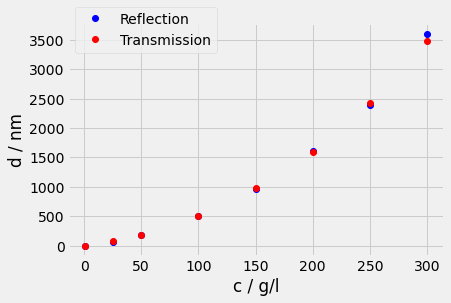
\includegraphics[width = 0.6\textwidth]{Bilder/Auswertung/Concentration/PlotReflTrans.png}
    \caption{Thickness of the films displayed as function of the concentration of the polymer solution $c$. The reflection measurements are depicted in blue, the transmission measurements in red.}
    \label{fig:ConcReflTrans}
\end{figure}

% discussion
The critical concentration $C^*$ is defined as the concentration for which the polymer chains start to overlap in the solution and the viscosity increases stronger with concentration.~\cite{Ruderer.2009} It seperates two regimes, which can be described as two lines.

\begin{equation}
    f(c) = \Theta_1(c - c^*) \cdot (m_2c + d_{02}) - [\Theta_0(c - c^*)-1] \cdot (m_1c+d_{01})
    \label{eq:twoLines}
\end{equation}

describes a function consisting of two lines, intersecting at the critical concentration $c^*$, where $\Theta_y(x)$ is the Heaviside function with $\Theta(x=0)=y$ and $m_{1/2}$ and $d_{01/02}$ are the slopes and offset for the first/second line. \par 

The resulting fit of the data points in figure \ref{fig:ConcReflTrans} with the function $f(c)$ and parameters $c^*$, $m_1$, $m_2$, $d_{01}$ and $d_{02}$ is displayed in figure \ref{fig:FitConc}. As well in the reflection measurements as in the transmission measurements a critical conentration of \par 
\centerline{\boxed{$c$^* = \SI{150}{\milli\gram\per\milli\litre}}} \par 
is found.

\begin{figure}[ht]
    \centering
    \begin{subfigure}[b]{0.49\textwidth}
        \centering
        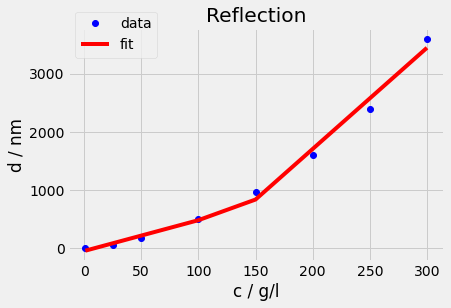
\includegraphics[width = \textwidth]{Bilder/Auswertung/Concentration/ReflFit.png}
    \end{subfigure}  
    \begin{subfigure}[b]{0.49\textwidth}
        \centering
        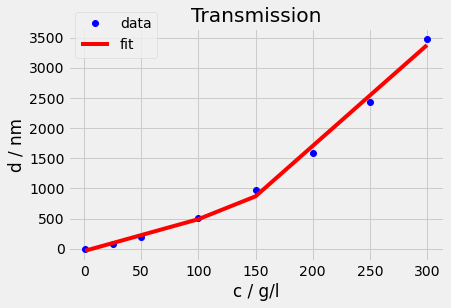
\includegraphics[width = \textwidth]{Bilder/Auswertung/Concentration/TransFit.png}
    \end{subfigure}  


    \caption{The film thickness in dependence of the concentration (blue dots) and fit using equation \ref{eq:twoLines}. As well in the reflection measurement (a) as in the transmission measuremtent (b) a critical concentration of $c^* =$ \SI{150}{\milli\gram\per\milli\litre} is found.}
    \label{fig:FitConc}
\end{figure}

The theoretical root-mean-square end-to-end distance can be calculated using 
\begin{equation}
    R_{rms} = \sqrt{C_{\infty}nl^2} = \sqrt{2C_{\infty}m_{PS}N_AM_S^{-1}l^2},
\end{equation}
where $C_{\infty} = 9.5$ is the charactaristic Flory ratio for PS, $l =$\SI{1.54}{\angstrom} is the length of a C-C-bond and the number of those bonds in the backbone of the polymer $n$ is obtained from 
\begin{equation}
    n = 2 \cdot \frac{m_{PS}}{m_S} = 2 \cdot \frac{m_{PS}N_A}{M_S}
\end{equation}
with the mass of the used PS $m_{PS} = $ \SI{35000}{\atomicmassunit}, Avogadro's constant $N_A$ and a molecular mass of the momomer styrene $M_S$ = \SI{104.15}{\gram\per\mol}.~\cite{Fetters.2007,Styrol} Using those values a root-mean-square end-to-end distance of \par
\centerline{\boxed{$R$_{rms} = \SI{123}{\angstrom}}} \par 
was obtained. \par
Another approach for calculating the root-mean-square end-to-end distance is using 
\begin{equation}
    R_{rms,exp} = 2.84 \cdot 10^{-8} \si{\mol^{-3}} \cdot (\frac{M_{PS}}{c^*})^\frac{1}{3}
\end{equation}
where $M_{PS}$ is the molecular mass of PS.~\cite{Daum.1969} This equation leads to \par 
\centerline{\boxed{$R$_{rms,exp} = \SI{175 \pm 10}{\angstrom}}} \par
Herefore, the critical concentration was being assumed to lie within \SIrange{125}{175}{\milli\gram\per\milli\litre} as the next measured concentrations from \SI{150}{\milli\gram\per\milli\litre} were \SI{100}{\milli\gram\per\milli\litre} and \SI{200}{\milli\gram\per\milli\litre}. 
%hallomats mäusssseeeeschreck, discussion why bigger
There are three common models, which describe the state of a polymer in solution: random coil, wormlike and rigid rods.~\cite{Ying.1987} For a random coil the root-mean-square end-to-end distance is given by \begin{equation}
    R_{rc} = 2 (\frac{M_{PS}}{c^*N_A})^\frac{1}{3} = 2.64 \cdot 10^{-8} \si{\mol^{-3}} \cdot (\frac{M_{PS}}{c^*})
\end{equation}
which leads to \par 
\centerline{\boxed{$R$_{rc} = \SI{146 \pm 24}{\angstrom}.}} \par
The length of a rigid rod can be calculated as
\begin{equation}
    L_r = \sqrt{2} \cdot (\frac{M_{PS}}{c^*N_A})^\frac{1}{3} = 1.67 \cdot 10^{-8} \si{\mol^{-3}} \cdot (\frac{M_{PS}}{c^*}),
\end{equation}
which leads to \par 
\centerline{\boxed{$L$_{r} = \SI{103 \pm 17}{\angstrom}.}} \par
The end-to-end distance of a wormlike structure $\widetilde{L}$ is calculated like a rigid rod. Therefore, 
\begin{equation}
    \widetilde{L} = L_r.
\end{equation} 
For obtaining the actual length of the chain $L_w$, the persistance length $L_p$ has to be taken in account: 
\begin{equation}
    \widetilde{L}^2 = L_w L_p
\end{equation}
$L_p$ can be calculated in the following way:
\begin{equation}
    L_p = \frac{L_k}{2} = \frac{C_{\infty}L_a}{2} = C_{\infty}L_{CC}\sin(\frac{\SI{109.5}{\degree}}{2}),
\end{equation}
where $L_k$ is the Kuhn-length, $L_{CC}$ is the length of a C-C-bond and $L_a$ is the actual end-to-end length of the polymer. The latter was calculated by assuming the backbone consisting only of C-C-bonds enclosing an angle of \SI{109.5}{\degree}. Following these equations one finds \par 
\centerline{\boxed{$L$_{w} = \SI{900 \pm 300}{\angstrom}.}} \par